\documentclass[aspectratio=169]{beamer}

%% Juego de caracteres usado en el archivo fuente: UTF-8
\usepackage{ucs}
\usepackage[utf8x]{inputenc}
\uselanguage{spanish}
%Para la identación del español
\usepackage[spanish]{babel}
\usepackage{animate}
\setbeamercovered{dynamic}
\useinnertheme{rectangles}

% There are many different themes available for Beamer. A comprehensive
% list with examples is given here:
% http://deic.uab.es/~iblanes/beamer_gallery/index_by_theme.html
% You can uncomment the themes below if you would like to use a different
% one:
%\usetheme{AnnArbor}
%\usetheme{Antibes}
%\usetheme{Bergen}
%\usetheme{Berkeley}
%\usetheme{Berlin}
%\usetheme{Boadilla}
%\usetheme{boxes}
%\usetheme{CambridgeUS}
%\usetheme{Copenhagen}
%\usetheme{Darmstadt}
%\usetheme{default}
%\usetheme{Frankfurt}
%\usetheme{Goettingen}
%\usetheme{Hannover}
%\usetheme{Ilmenau}
%\usetheme{JuanLesPins}
%\usetheme{Luebeck}
\usetheme{Madrid}
%\usetheme{Malmoe}
%\usetheme{Marburg}
%\usetheme{Montpellier}
%\usetheme{PaloAlto}
%\usetheme{Pittsburgh}
%\usetheme{Rochester}
%\usetheme{Singapore}
%\usetheme{Szeged}
%\usetheme{Warsaw}

%Para la identación del español
\usepackage[spanish]{babel}

\title{Infraestructura de red de nodos cifradores/descifradores AES basada en ApSoC}

% A subtitle is optional and this may be deleted
%\subtitle{Optional Subtitle}

\author{Jesús Rodríguez Heras}
% - Give the names in the same order as the appear in the paper.
% - Use the \inst{?} command only if the authors have different
%   affiliation.

%\institute[Escuela Superior de Ingeniería] % (optional, but mostly needed)
%{
%  \inst{1}%
%  Department of Computer Science\\
%  University of Somewhere
%  \and
%  \inst{2}%
%  Department of Theoretical Philosophy\\
%  University of Elsewhere}
% - Use the \inst command only if there are several affiliations.
% - Keep it simple, no one is interested in your street address.

\date{24 de septiembre de 2020}
% - Either use conference name or its abbreviation.
% - Not really informative to the audience, more for people (including
%   yourself) who are reading the slides online

%\subject{Theoretical Computer Science}
% This is only inserted into the PDF information catalog. Can be left
% out. 

% If you have a file called "university-logo-filename.xxx", where xxx
% is a graphic format that can be processed by latex or pdflatex,
% resp., then you can add a logo as follows:

% pgfdeclareimage[height=0.5cm]{university-logo}{university-logo-filename}
% \logo{\pgfuseimage{university-logo}}

% Delete this, if you do not want the table of contents to pop up at
% the beginning of each subsection:
\AtBeginSection[]
{
  \begin{frame}<beamer>{Índice}
    \tableofcontents[currentsection]
  \end{frame}
}
%\AtBeginSubsection[]
%{
%	\begin{frame}<beamer>{Índice}
%	\tableofcontents[currentsection,currentsubsection]
%\end{frame}
%}

% Let's get started
\begin{document}

\begin{frame}
  \titlepage
%  \begin{center}
%  Luis Gutiérrez Flores\\
%Nicolás Ruiz Requejo\\
%Jesús Rodríguez Heras\\
%Arantzazu Otal Alberro\\
%Alejandro Segovia Gallardo\\
%Alejandro José Caraballo García\\
%Gabriel Fernando Sánchez Reina	
%  \end{center}
  
\end{frame}

\begin{frame}{Índice}
%\small
\tableofcontents
\end{frame}
%\normalsize

\section{Introducción}
\subsection{Objetivos}
\begin{frame}{Objetivos}
%\textcolor{red}{Aquí hablaríamos de lo que son los objetivos al igual que en la memoria pero mucho más esquemático para que me permita hablar más que lo que es la lectura de la diapositiva por parte del tribunal}
Los objetivos generales de este proyecto son los siguientes:
\begin{itemize}
	\item Diseñar red de nodos basada en la tecnología ApSoC.
	\item Establecer comunicación entre nodos de la red.
	\item Aportar información a un fichero común de forma secuencial.
\end{itemize}
\end{frame}

\subsection{Descripción}
\begin{frame}{Descripción}
%\textcolor{red}{Hablamos de la descripción como en la memoria}
\begin{block}{Nodos}
	Los nodos de la red serán tarjetas de desarrollo Zybo Zynq 7010.
\end{block}
\begin{figure}[h]
	\centering
	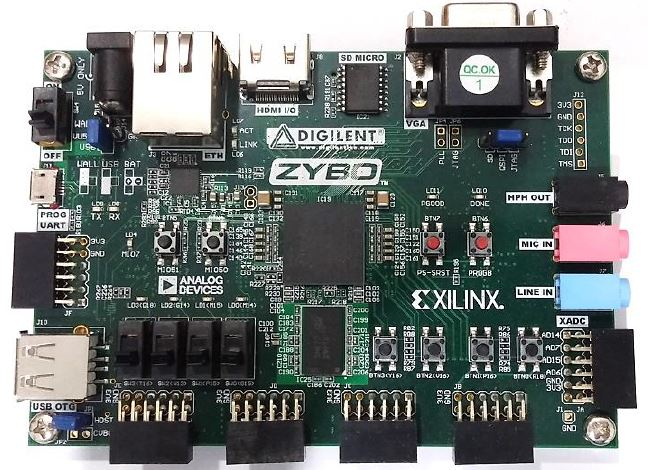
\includegraphics[scale=0.4]{Fotos/zybo.jpg}
\end{figure}
\end{frame}



\subsection{Alcance}
\begin{frame}{Alcance}
\begin{block}{Infraestructura de red}
	\begin{itemize}
		\item Instalación de Linux en las tarjetas.
		\item Interconexión física de los elementos de la red.
		\item Desarrollo de scripts automáticos.
		\item Creación y ejecición de pruebas.
	\end{itemize}
\end{block}
\end{frame}
%\begin{frame}{Alcance}
%\textcolor{red}{Hablamos de lo que consiste el alcance, como en la memoria.\\Realmente lo he estructurado todo como en la memoria con la idea de tener una guía que seguir y que todo vaya, más o menos, cogido de la mano.}
%El proyecto contará con los siguientes apartados:
%\begin{itemize}
%	\item 
%\end{itemize}
%\end{frame}

\section{Metodología}
\subsection{Marco teórico}
\begin{frame}{Marco teórico}
\begin{itemize}
	\item El punto de partida de este proyecto son las tarjetas de desarrollo Zybo Zynq 7010 que actuarán como nodos de la red.
	\item Se establecerán comunicaciones entre ellas para enviar un fichero recolector de información.
\end{itemize}
\end{frame}

\subsection{Tecnologías a utilizar}
\begin{frame}{Tecnologías a utilizar}
\begin{block}{Componentes}
	\begin{itemize}
		\item Ordenador central (monitor).
		\item Tarjeta Zybo Zynq 7010.
		\item Switch.
	\end{itemize}
\end{block}
\begin{figure}[h]
\centering
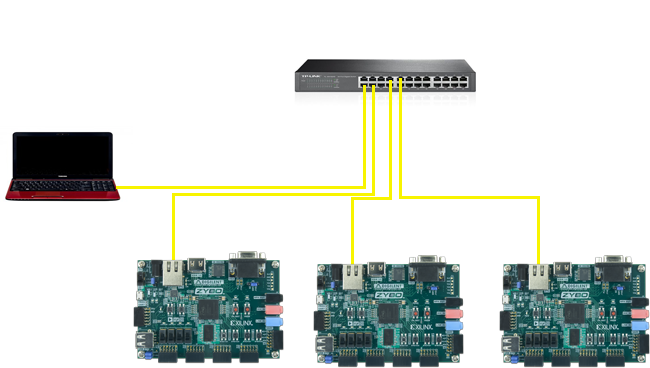
\includegraphics[scale=0.3]{Fotos/RedCompleta.png}
\end{figure}
\end{frame}

\subsection{Análisis del sistema}
\begin{frame}{Análisis del sistema}
\begin{block}{Ordenador central}
	Creará el fichero inicial y será el punto de partida y final de la cadena.
\end{block}
\begin{block}{Nodos}
	Tendrán instalado un sistema operativo Linux para la gestión de ficheros y las funcionalidades de red.
\end{block}
\begin{block}{Switch}
	No tendrá ninguna configuración adicional.
\end{block}
\end{frame}

\begin{frame}{Análisis del sistema}
	Para la transmisión del fichero de datos a través de la red, usaremos el protocolo SSH y una serie de scripts:
	\begin{block}{Scripts}
		\begin{itemize}
			\item \texttt{Inicio.sh}
			\item \texttt{Lanzador.sh}
			\item \texttt{Automatico.sh}
			\item \texttt{Recibiendo.sh}
			\item \texttt{Cristian.sh}
			\item \texttt{Enviando.sh}
			\item \texttt{Borrar.sh}
		\end{itemize}
	\end{block}
\end{frame}

\begin{frame}{Análisis del sistema}
	La secuencia de trabajo de estos scripts será la siguiente:
	\begin{figure}[h]
		\centering
		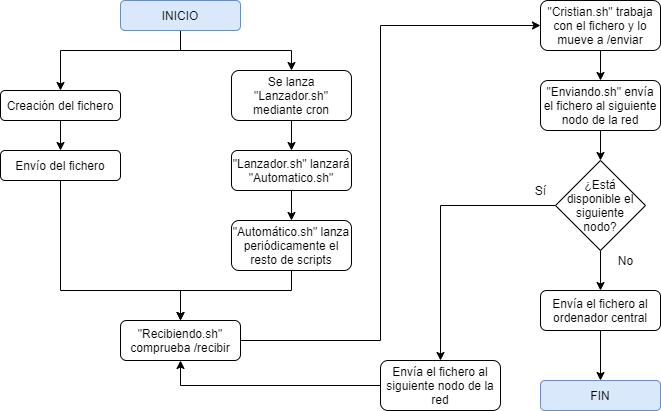
\includegraphics[scale=0.45]{Fotos/CadenaScriptsAncho.png}
	\end{figure}
\end{frame}

\subsection{Diseño y desarrollo}
\begin{frame}{Diseño y desarrollo}
\begin{itemize}
	\item Todos los dispositivos de la red han de estar conectados al switch y tener una IP fija.
	\item El proceso de comunicación se inicia en el ordenador central (monitor).
	\item Los nodos reciben el fichero, añaden información y lo envían al siguiente nodo de la red.
	\item El proceso de comunicación finaliza cuando el fichero es recibido por el monitor.
\end{itemize}
\end{frame}

\subsection{Pruebas del sistema}
\begin{frame}{Pruebas del sistema}
\begin{block}{Prueba de conexión}
	Lanzamos el script \texttt{Inicio.sh} en el ordenador central.
	\begin{figure}[h]
		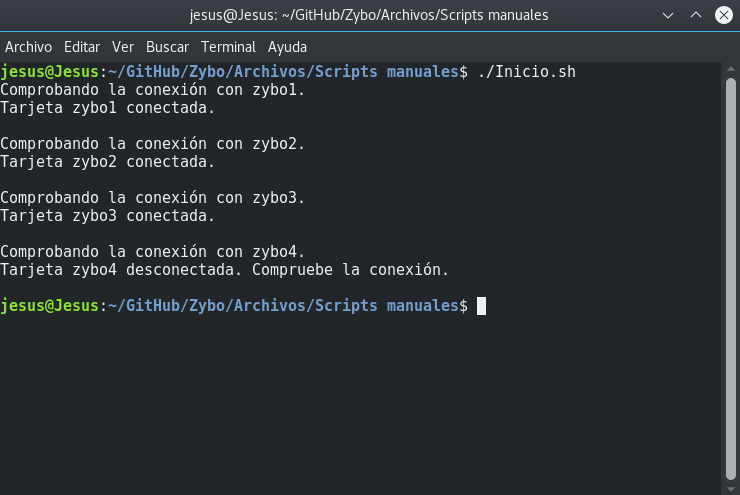
\includegraphics[scale=0.3]{Fotos/Prueba_Inicio_sh.png}
	\end{figure}
\end{block}
\end{frame}

\begin{frame}{Pruebas del sistema}
\begin{block}{Prueba de funcionamiento (I)}
	Creamos el fichero de pruebas y lo enviamos al primer nodo de la red.
	\begin{figure}[h]
		\centering
		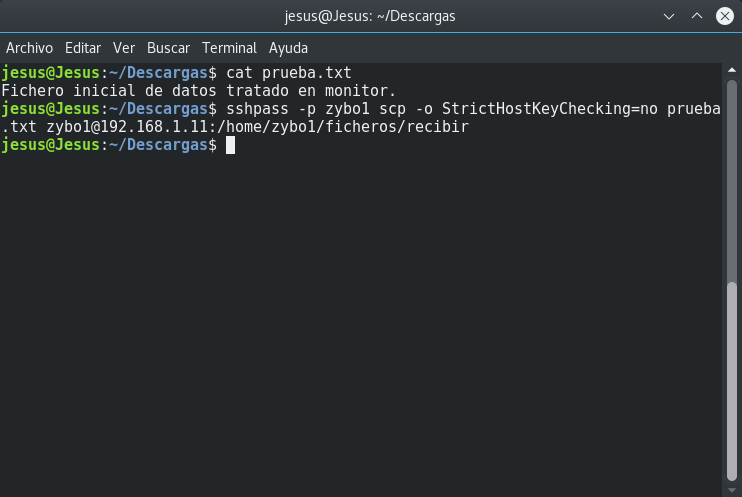
\includegraphics[scale=0.3]{Fotos/Fichero_inicial_en_PC.png}
	\end{figure}
\end{block}
\end{frame}

\begin{frame}{Pruebas del sistema}
\begin{block}{Prueba de funcionamiento (II)}
	Comprobamos el paso del fichero por la tarjeta Zybo.
	\begin{figure}[h]
		\centering
		\includegraphics[scale=0.3]{Fotos/Fichero_en_zybo1.png}
	\end{figure}
\end{block}
\end{frame}

\begin{frame}{Pruebas del sistema}
\begin{block}{Prueba de funcionamiento (III)}
	Una vez completada la cadena de nodos, comprobamos el fichero en el monitor.
	\begin{figure}[h]
		\centering
		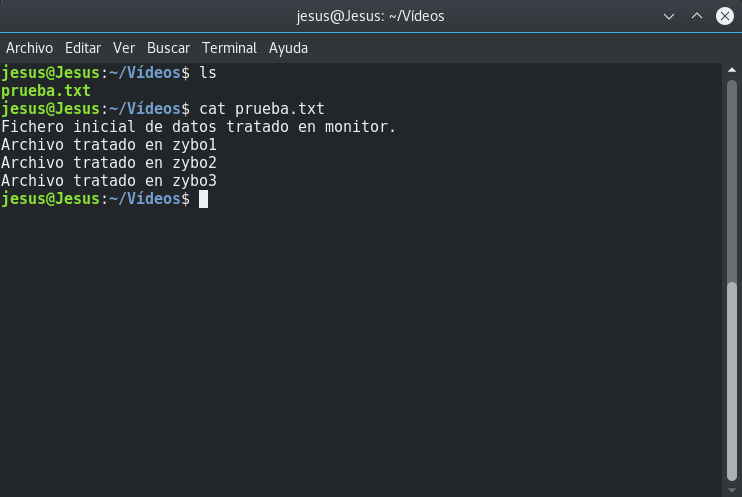
\includegraphics[scale=0.3]{Fotos/Fichero_final_en_PC.png}
	\end{figure}
\end{block}
\end{frame}

\section{Conclusiones y trabajo futuro}
\subsection{Conclusiones}
\begin{frame}{Conclusiones}
\begin{block}{Escenario de trabajo 1}
	Todos los nodos están conectados correctamente a la red.
	\begin{figure}[h]
		\centering
		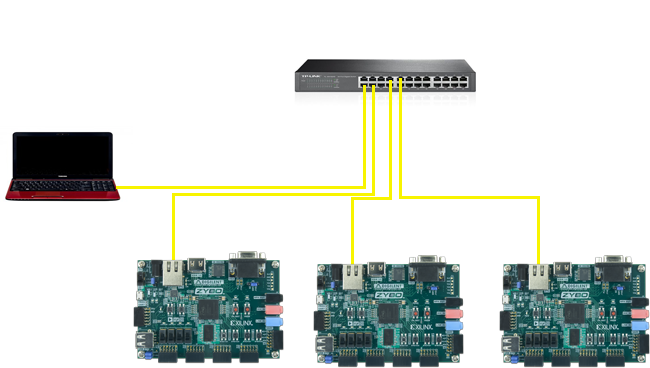
\includegraphics[scale=0.4]{Fotos/RedCompleta.png}
	\end{figure}
\end{block}
\end{frame}

\begin{frame}{Conclusiones}
\begin{block}{Escenario de trabajo 2}
	Un nodo intermedio se encuentra desconectado.
	\begin{figure}[h]
		\centering
		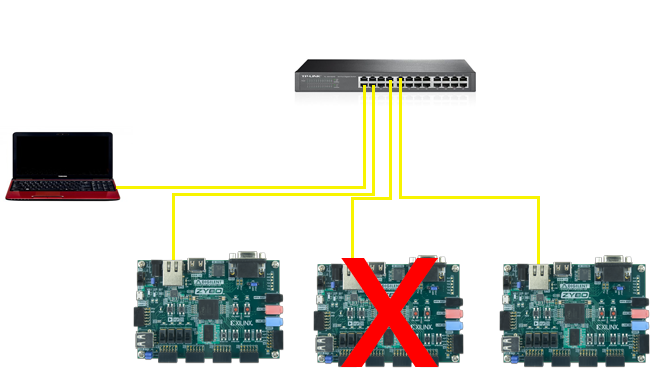
\includegraphics[scale=0.4]{Fotos/RedSinNodo2.png}
	\end{figure}
\end{block}
\end{frame}

\begin{frame}{Conclusiones}
\begin{block}{Escenario de trabajo 3}
	El primer nodo está desconectado.
	\begin{figure}[h]
		\centering
		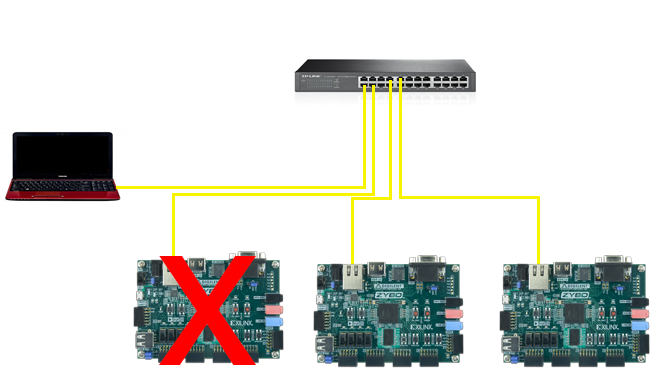
\includegraphics[scale=0.4]{Fotos/RedSinNodo1.png}
	\end{figure}
\end{block}
\end{frame}

\subsection{Trabajo futuro}
\begin{frame}{Trabajo futuro}
\begin{itemize}
	\item Cambiar cadena de conexiones a aleatorio.
	\item Completar el trabajo de cifrado/descifrado incluyendo el IP cifrador/descifrador AES de Cristian Ambrosio Costoya.
	\item Implementación de un módulo IEEE 802.11 para conexiones inalámbricas.
\end{itemize}
\end{frame}

\end{document}


